\documentclass[article, a4paper, amsfonts, amssymb, amsmath, reprint, showkeys, nofootinbib, twoside]{revtex4-1}
%%%%%%%%%%%%%%%%%%%%%%%%%%%%%
\usepackage[spanish]{babel}
\usepackage[utf8]{inputenc}
\usepackage[colorinlistoftodos, color=green!40, prependcaption]{todonotes}
%\input{preamble}
%%%%%%%%%%%%%%%%%%%%%%%%%%%%%
\usepackage{color}
\usepackage{boldline}
\usepackage{fancyhdr}
\usepackage{tcolorbox}
\usepackage{enumitem} % para unificar numeracion en los enumerate
\usepackage{caption}
\usepackage{qrcode}
%%%%%%%%%%%%%%%%%%%%%%%%%%%%%
\usepackage[pdftex, pdftitle={Article},pdfauthor={Author},pagebackref=true,colorlinks=true,linkcolor=blue,urlcolor=blue,citecolor=red]{hyperref} % For hyperlinks in the PDF
%\setlength{\marginparwidth}{2.5cm}

\bibliographystyle{apsrev4-1}
\definecolor{saltalafisica}{HTML}{2D947F}

\begin{document}
%%%%%%%%%%%%%%%%%%%%%%%%%%%%%
\title{ \LARGE \textcolor{saltalafisica}{GUÍA DE LENTES ESFÉRICAS} \\ NIVEL FUNDAMENTOS \\ \hrulefill \\ }

\author{\large \textbf{\textcolor{saltalafisica}{La Física al Alcance de Todos - Prof. Daniel Córdoba} }}
\homepage{https://saltalafisica.github.io/}
\affiliation{}
\begin{abstract}
\end{abstract}
%\keywords{first keyword, second keyword, third keyword}
%%%%%%%%%%%%%%%%%%%%%%%%%%%%%
\maketitle
%%%%%%%%%%%%%%%%%%%%%%%%%%%%%
\thispagestyle{fancy}
\fancyhead[L]{
    \begin{picture}(0,0)
        \put(0,-70){\includegraphics[width=3cm, height=3cm]{Imagenes/gofito_sinfondo.png}}
    \end{picture}
}
\renewcommand{\headrulewidth}{0.pt}
\pagestyle{plain}
%%%%%%%%%%%%%%%%%%%%%%%%%%%%%

\definecolor{fondocuadros}{RGB}{236,231,231}


\begin{center}
    Accede a todas las guías de problemas desde el siguiente código:

    %\qrset{nolink, height=4cm, padding}
    %\qrcode{https://saltalafisica.ar/n1/guias/}
    
\includegraphics[height=3cm]{Imagenes/qr.jpeg}
\end{center}

%\center{\Large \bf Preguntas conceptuales}

\begin{center}
    {\Large \bf Preguntas conceptuales}
\end{center}

\begin{enumerate}[start=1, label=\textbf{\arabic*.}]
    \item Complete las figuras de este ejercicio trazando las trayectorias de los rayos luminosos indicados, luego de atravesar las lentes. La distancia focal de ambas es igual a $5 \text{ cm}$.

          \begin{figure}[h!]
              \centering
              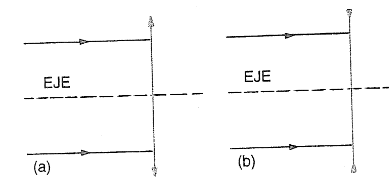
\includegraphics[width=0.7\linewidth]{Imagenes/ej1.png}
              \caption*{Ejercicio 1}
              %\label{fig:placeholder}
          \end{figure}

    \item En la figura de este ejercicio se tienen dos lentes, las posiciones de sus focos y los rayos luminosos que salen de ellas. Trace en la figura los rayos incidentes que produjeron tales rayos emergentes.

          \begin{figure}[h!]
              \centering
              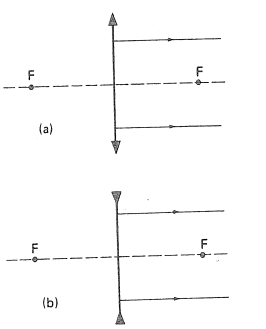
\includegraphics[width=0.8\linewidth]{Imagenes/ej2.png}
              \caption*{Ejercicio 2}
              %\label{fig:placeholder}
          \end{figure}

    \item En la figura de este ejercicio se ve una lente de plástico, cuyo índice de refracción es $n = 1.7$, sumergida en dos medios con índices de refracción $n_1$ y $n_2$.
          \begin{enumerate}[label=\emph{\alph*})]
              \item Esta lente, al aire, ¿es convergente o divergente?
              \item Observando las trayectorias de los rayos luminosos que se señalan en la figura, diga si el valor de $n_1$ es mayor, menor o igual a $1.7$.
              \item Y el valor de $n_2$, ¿es mayor, menor o igual a $1.7$?
          \end{enumerate}

          \begin{figure}[h!]
              \centering
              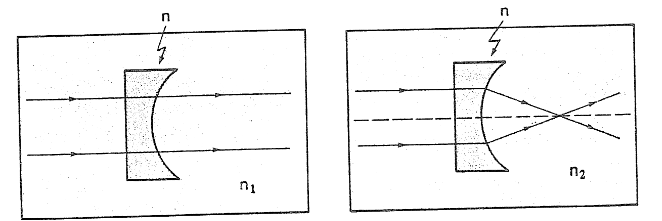
\includegraphics[width=1\linewidth]{Imagenes/ej3.png}
              \caption*{Ejercicio 3}
              %            \label{fig:placeholder}
          \end{figure}

    \item La figura de este ejercicio muestra un objeto $AB$ colocado frente a una lente convergente, y las posiciones de los focos de ésta.
          \begin{enumerate}[label=\emph{\alph*})]
              \item Trace el diagrama que permita localizar la imagen de este objeto proporcionada por la lente.
              \item La imagen obtenida, ¿es real o virtual? ¿Es derecha o invertida? ¿Y mayor o menor que el objeto?
          \end{enumerate}

          \begin{figure}[h!]
              \centering
              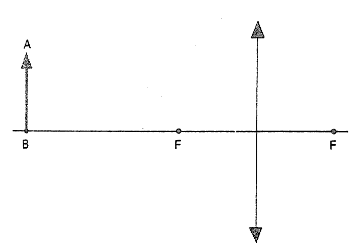
\includegraphics[width=0.65\linewidth]{Imagenes/ej4.png}
              \caption*{Ejercicio 4}
              %            \label{fig:placeholder}
          \end{figure}

          \vspace{1 cm}

    \item Suponga que el objeto del ejercicio anterior se acercara a la lente y quedara situado a una distancia $D_o$ comprendida entre $f$ y $2f$.
          \begin{enumerate}[label=\emph{\alph*})]
              \item Trace el diagrama de localización de la imagen del objeto.
              \item Entonces, conforme un cuerpo es acercado a una lente convergente (sin sobrepasar al foco), ¿su imagen permanece real? ¿Se acerca o se aleja de la lente? ¿Aumenta o disminuye de tamaño?
          \end{enumerate}

    \item Considere de nuevo la lente y el objeto del Ejercicio 4. Sitúe ahora a $AB$ entre el foco y la lente.
          \begin{enumerate}[label=\emph{\alph*})]
              \item Localice mediante un diagrama la imagen del objeto en esta posición.
              \item Describa las características de esta imagen.
          \end{enumerate}

    \item Un objeto $AB$ se encuentra frente a una lente divergente, como muestra la figura de este ejercicio.
          \begin{enumerate}[label=\emph{\alph*})]
              \item Trace un diagrama para obtener la imagen de este objeto y describa las características de su imagen.
              \item Acerque el objeto y colóquelo entre el foco y la lente. Trace el diagrama, localice la imagen y describa sus características.
              \item Observando los diagramas que trazó en (a) y (b), ¿a qué conclusión puede llegar acerca de la naturaleza y el tamaño de la imagen proporcionada por una lente divergente?
          \end{enumerate}

          \begin{figure}[h!]
              \centering
              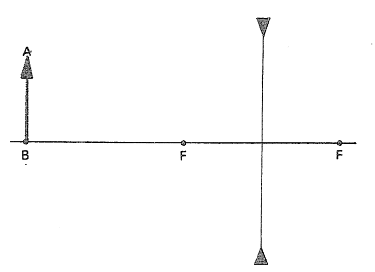
\includegraphics[width=0.8\linewidth]{Imagenes/ej6.png}
              \caption*{Ejercicio 7}
              %\label{fig:placeholder}
          \end{figure}

          \newpage

          \begin{center}
              {\Large \bf Ejercicios}
          \end{center}

          \vspace{1 cm}

    \item En el Ejercicio 4 suponga que la distancia focal de la lente es $f = 4 \text{ cm}$, y que el objeto $AB$ se encuentra situado a una distancia $D_o = 12 \text{ cm}$.
          \begin{enumerate}[label=\emph{\alph*})]
              \item Usando la ecuación de las lentes, determine la distancia, $D_i$ de la imagen a la lente.
              \item ¿Cuál es el aumento proporcionado por la lente?
              \item ¿Qué significado tiene la respuesta de la pregunta (b)?
              \item Sus contestaciones en este ejercicio, ¿concuerdan con el diagrama trazado en el Ejercicio 4?
          \end{enumerate}

    \item En la figura del Ejercicio 7 suponga que la distancia focal de la lente es de $4 \text{ cm}$ y que el objeto se encuentra a $12 \text{ cm}$ de ella.
          \begin{enumerate}[label=\emph{\alph*})]
              \item Calcule la distancia $D_i$ de la imagen a la lente.
              \item Determine el aumento proporcionado por esta última.
              \item Si el tamaño del objeto es $AB = 10 \text{ cm}$, ¿cuál es el tamaño de la imagen $A'B'$?
          \end{enumerate}



\end{enumerate}
\end{document}
